\newpage
\section{Metodologia Experimental}

\subsection{Materiais}
O material utilizado foi:
\begin{itemize}
\item Computador.
\item Software Orcad.

\subsection{Métodos}
\end{itemize}
Para execução do experimento, faz-se necessário executar os seguintes passos (com base no circuito da Figura \ref{f_sch}, e a tabela com valores dos componentes Tabela \ref{tab:componentes}):

\begin{figure}[H]
    \centering
        \caption{Oscilador LC com buffer.}\label{f_sch}
    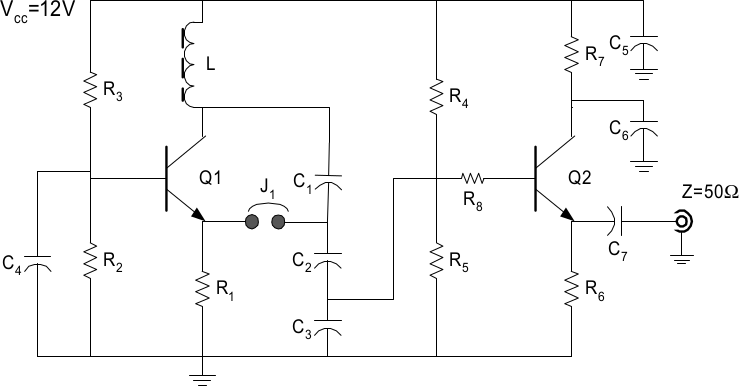
\includegraphics[scale=0.3]{Imagens/sch.png}

    \small Fonte: Me. Jaime Laelson Jacob, 2016.
\end{figure}

\begin{itemize}
\item calcular o valor do indutor L para uma frequência de 4MHz;
\item simular o circuito mostrado na figura \ref{f_sch} com o software Orcad;
\item analisar a forma de onda no estágio oscilador e na saída (frequência, amplitude, distorção);
\item calcular a potência entregue a carga;
\item simular uma ponteira de osciloscópio e mensurar a variação da frequência de saída quando a ponteira é colocada nos pontos:
    \begin{enumerate}[label=\roman{*}]
        \item Saída do oscilador (emissor de Q2);
        \item Coletor de Q1;
        \item Em J1;
        \item Sobre C1.
    \end{enumerate}
\item medir o conteúdo espectral da saída e montar uma tabela relacionando as harmônicas presentes e respectivas potências (relativas).
\item variar a tensão de saída em +- 20\% e verificar se há alteração na frequência de saída e calcular a estabilidade relativa em partes por milhão por volts.
\end{itemize}


\begin{table}[H]
    \begin{center}
        \caption{Valores dos componentes para o circuito da Figura \ref{f_sch}}        \label{tab:componentes}
        \begin{tabular}{c|c|c|c}
            \hline
            $R_1 = 3,9k\Omega$ & $R_6 = 330\Omega$ & $C_1 = 470pF$ & $C_6 = 10nF$ \\
            $R_2 = 3,9k\Omega$ & $R_7 = 100\Omega$ & $C_2 = 10nF$ & $C_7 = 10nF$ \\
            $R_3 = 22k\Omega$ & $R_8 = 470\Omega$ & $C_3 = 8.2nF$ & $Q_1 = BF254$ \\
            $R_4 = 3,9k\Omega$ & & $C_4 = 10nF$ & $Q_2 = BF254$ \\
            $R_5 = 8,2k\Omega$ & & $C_5 = 100nF$ & \\
            \hline
        \end{tabular}
        
        \small Fonte: Me. Jaime Laelson Jacob, 2016.
    \end{center}
\end{table}
